%% Author_tex.tex
%% V1.0
%% 2012/13/12
%% developed by Techset
%%
%% This file describes the coding for rsproca.cls

\documentclass[openacc]{rsproca_new}%%%%where rsproca is the template name
\usepackage{subcaption}
\usepackage[thinc]{esdiff} % for derivatives
\usepackage{empheq} % boxed equations
\usepackage{amsmath}

\definecolor{myboxcolor}{rgb}{0.96, 0.96, 0.96}
\newcommand*\mybox[1]{%
\colorbox{myboxcolor}{\hspace{1em}#1\hspace{1em}}}

\usepackage{xspace}
\newcommand\thedata {$\{(t_i,h_{\text{obs}, i})\}_{i=1}^{N}$\xspace}
\newcommand\thedatanomath {\{(t_i,h_{\text{obs}, i})\}_{i=1}^{N}}
\newcommand\themodel {$h(t; h_0, \boldsymbol \alpha, \boldsymbol\theta)$\xspace}
\newcommand\themodelnomath {h(t; h_0, \boldsymbol \alpha, \boldsymbol\theta)}
\newcommand\thevars{h_0, \boldsymbol \alpha, \boldsymbol \theta, \sigma^2}

% from empheq pkg
\definecolor{shadecolor}{rgb}{0.97, 0.97, 1.0}
\definecolor{titlecolor}{rgb}{0.96, 1.0, 0.98}
\newsavebox{\mysaveboxM} % M for math
\newsavebox{\mysaveboxT} % T for text
\newcommand*\Garybox[2][Example]{%
\sbox{\mysaveboxM}{#2}%
\sbox{\mysaveboxT}{\fcolorbox{black}{titlecolor}{#1}}%
\sbox{\mysaveboxM}{%
\fcolorbox{black}{shadecolor}{%
\makebox[\linewidth-10em]{\usebox{\mysaveboxM}}%
}%
}%
\usebox{\mysaveboxM}%
\makebox[0pt][r]{%
\makebox[\wd\mysaveboxM][c]{%
\raisebox{\ht\mysaveboxM-0.5\ht\mysaveboxT
+1.6\dp\mysaveboxT-0.5\fboxrule}{\usebox{\mysaveboxT}}%
}%
}%
}


\usepackage{tcolorbox} 
\tcbuselibrary{breakable}
\newtcolorbox[auto counter
]{mytcbox}[2][]{
% title=Box~\thetcbcounter: #2,#1,
title=#2, #1,
colback=white,
colframe=black,
fonttitle=\bfseries,
parbox=false
}


%%%% *** Do not adjust lengths that control margins, column widths, etc. ***

%%%%%%%%%%% Defining Enunciations  %%%%%%%%%%%
\newtheorem{theorem}{\bf Theorem}[section]
\newtheorem{condition}{\bf Condition}[section]
\newtheorem{corollary}{\bf Corollary}[section]
%%%%%%%%%%%%%%%%%%%%%%%%%%%%%%%%%%%%%%%%%%%%%%%

%%%%% Please insert respective article type here %%%%
\titlehead{Research}

\begin{document}

%%%% Article title to be placed here
% \title{Bayesian inference of the shape of an object inside of a gravity-drained tank}
%\title{Inferring the shape of a solid inside a gravity-drained tank from liquid level time series data}
\title{Inferring the shape of a solid inside a liquid-holding tank from its liquid level as it drains}


\author{%%%% Author details
Gbenga Fabusola$^{1}$, 
Cory M. Simon$^{1}$
}

%%%%%%%%% Insert author address here
\address{$^{1}$School of Chemical, Biological, and Environmental Engineering. Oregon State University. Corvallis, OR, USA.
% $^{2}$Second author address\\
}

%%%% Subject entries to be placed here %%%%
\subject{applied mathematics, chemical engineering}

%%%% Keyword entries to be placed here %%%%
\keywords{inverse problems, Bayesian statistical inversion, Torricelli's law}

%%%% Insert corresponding author and its email address}
\corres{Cory M. Simon\\
\email{cory.simon@oregonstate.edu}}

%%%% Abstract text to be placed here %%%%%%%%%%%%
\begin{abstract}
In engineering, we often encounter an open-top, liquid-holding tank draining via gravity-driven flow through a small orifice in its side. 
Torricelli's law and a mass balance give a differential equation model governing the dynamics of the liquid level in the tank. 
Herein, we consider the inverse problem of leveraging this model to infer the shape of an exogenous solid, heavy object inside of a tank draining of liquid, using measurements of the liquid level over time. (Because the object displaces liquid, the rate of decrease of the liquid level provides information about the cross-sectional area of the object at that height; as the liquid level drops, we ``scan'' the area of the object as a function of height.) To quantify uncertainty about the shape of the object, we employ Bayesian statistical inversion for reconstructing the object's cross-sectional area as a function of height. 

In our experimental setup, a small, open-top tank 
% (an inverted, truncated cone with a rounded rectangle base) 
drains of water through a small orifice in its side; a liquid level sensor collects time series data of the water level. 
First, we calibrate and test our forward model of the dynamics of the water level using data from two drainage experiments without an object inside of the tank. Second, we conduct a drainage experiment with an object inside the tank, then leverage the calibrated forward model and the liquid level time series data to predict (i.e., obtain a posterior distribution for) the shape of the object inside the tank with quantified uncertainty.
Our approach may be practically useful to infer the shape of an unknown object, or the porosity of packed particles, inside of an opaque tank that gives access to liquid level measurements. 
\newline

\begin{center}
	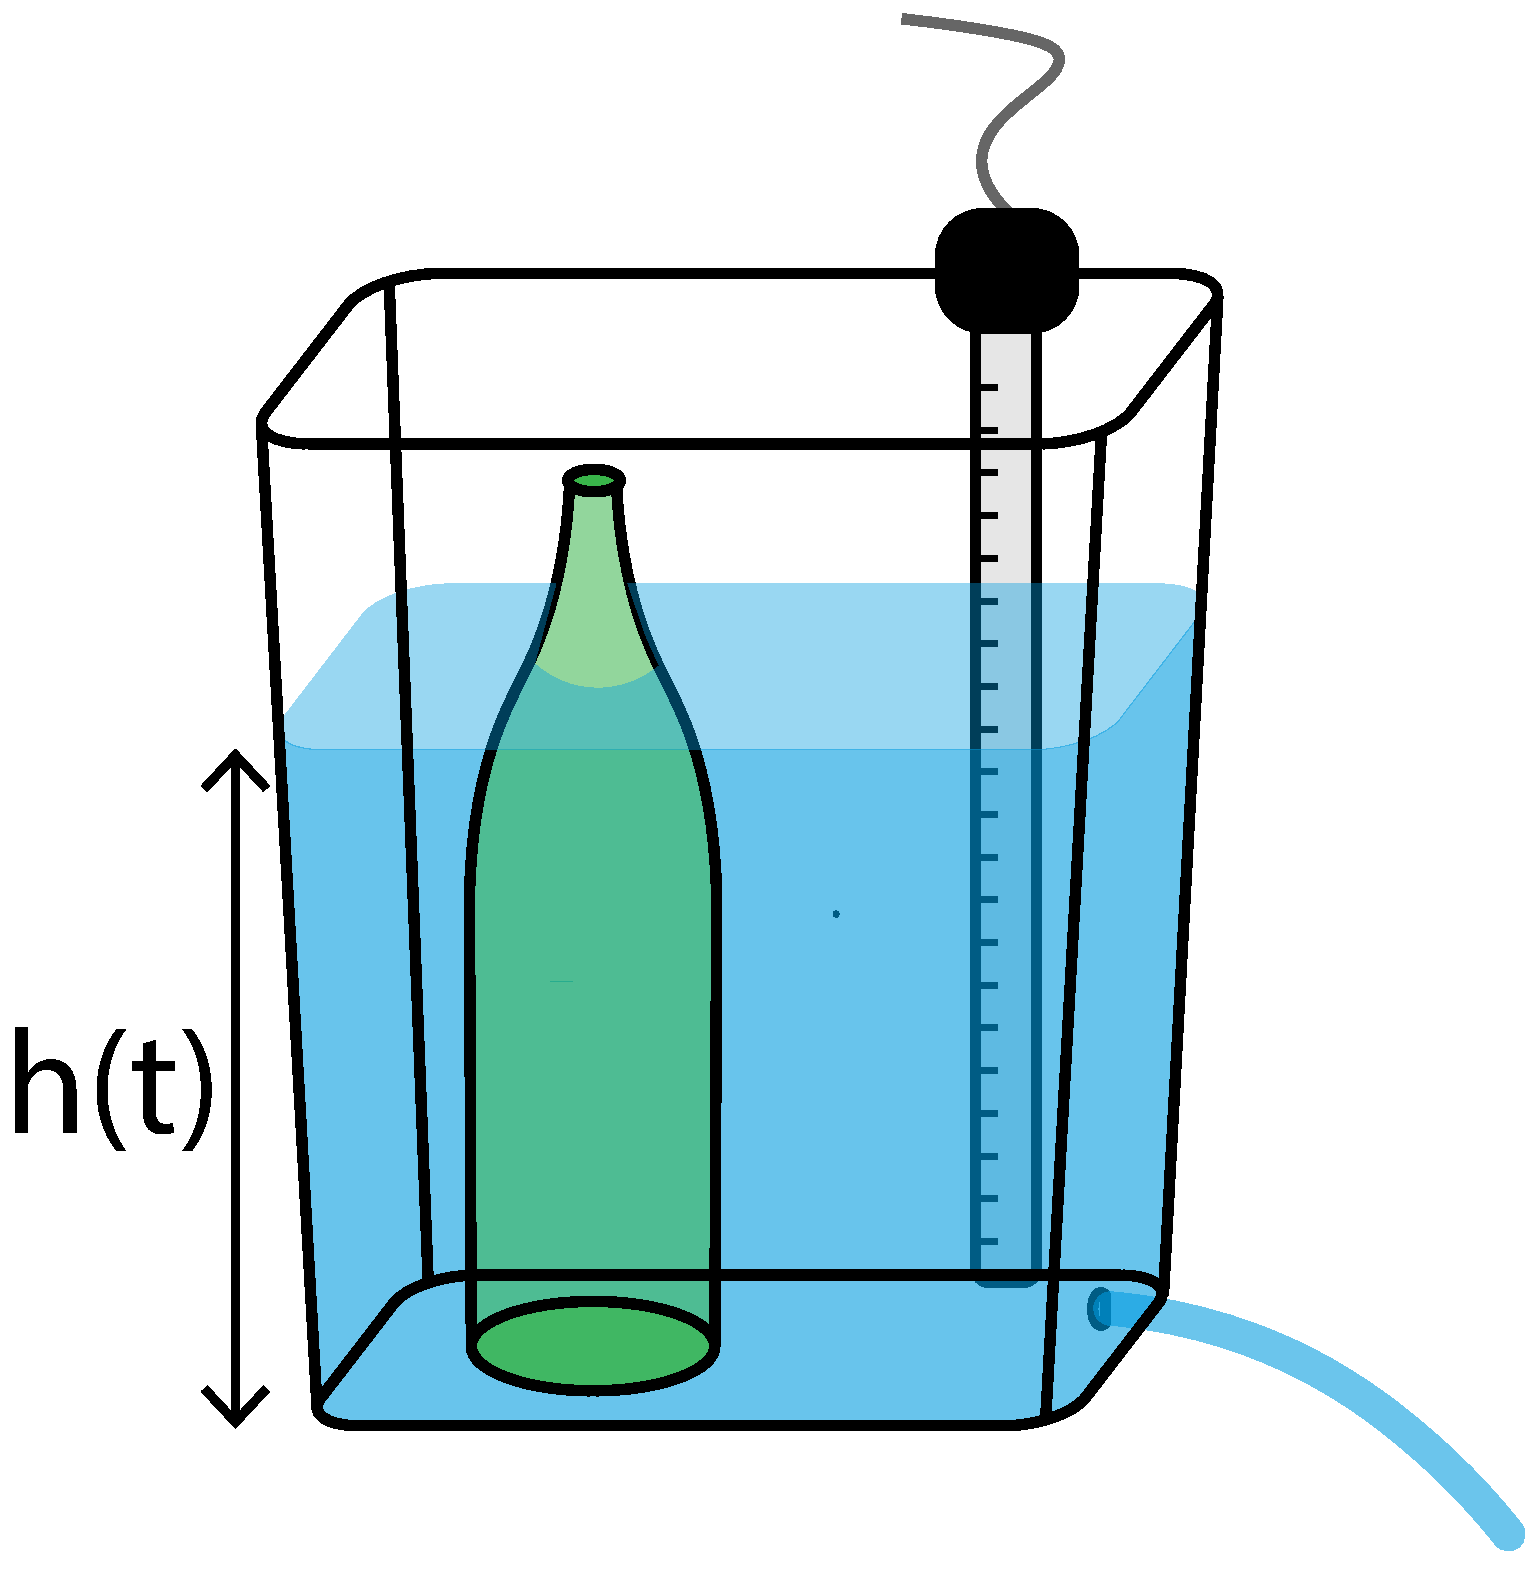
\includegraphics[height=0.375\textwidth]{../tank_geometry/tank_w_bottle.pdf}
	\includegraphics[height=0.375\textwidth]{../toy_h_w_object.pdf}
\end{center}

\absbreak % unclear why this is needed


\end{abstract}
%%%%%%%%%%%%%%%%%%%%%%%%%%%



\rsbreak

%%%%%%%%%% Insert the texts which can accomdate on firstpage in the tag "fmtext" %%%%%

\section{Introduction}
Throughout engineering and the applied sciences, we encounter a liquid-holding tank, draining via gravity-driven flow through a small orifice.
Mathematical models of the dynamics of the liquid level in a draining tank are useful for designing the geometry of the tank and orifice, predicting the emptying time, forecasting the outlet flow rate, controlling the liquid level by manipulating an input stream, and inferring the liquid level from the outlet flow rate \cite{d2021torricelli,seborg2016process,groetsch1993inverse,groetsch1999inverse}.

\begin{mytcbox}[label=box:waterclocks, breakable]{Ancient water clocks}
Interestingly, ancient societies (e.g. ancient Greece) exploited the empirically predictable dynamics of the water level in a draining container to measure and display the passage of time.
Specifically, the outflow \emph{clepsydra}, Greek for ``water thief'', was an open-top container with a small hole near its bottom and graduated markings on the inside. 
Filled with water then allowed to drain, the elapsed time was indicated by the liquid level with respect to the markings on the inside. \cite{bedini1962compartmented,hwang2021historical,ritner2016oriental,hejun1987research,schomberg2018karnak,mills1982newton}
The preserved Karnak clepsydra from $\sim$1300 BC \cite{schomberg2018karnak} is an inverted truncated cone. Notably, this geometry does not provide a constant rate of decrease in the water level; perhaps, though, its wider top was intended to compensate for faster outflow at higher water levels. An inverse problem pertaining to an outflow clepsydra is: what clepsydra shape provides a constant rate of decrease in the water level as it drains?
(Such a clepsydra may be obtained via a solid of revolution about the vertical axis such that the radius is proportional to the quartic root of the height. \cite{mills1982newton,d2021torricelli})
\end{mytcbox}
%Draining tanks have been studied since ancient times, as evidenced by water clocks in ancient Egypt, Greece, India, and China.
%The water clock, or clepsydra (Greek for ''water thief''), of the outflow design consisted of an open-top container, filled with water at some reference time, with a small orifice for outflow near its bottom.

%The geometry of an ideal clepsydra would produce a constant rate of decrease in the liquid level. However, the geometry of e.g. the preserved Karnak clepsydra from $\sim$1300 BC \cite{schomberg2018karnak}, an inverted truncated cone, does not. Though, perhaps, its wider top was intended to compensate for the faster outflow when the liquid level is higher.

% Italian physicist and mathematician 
Evangelista Torricelli (1608-1647) made a fundamental observation for mathematical modeling the liquid level in a tank draining via gravity-driven flow through a small orifice: the velocity $v$ at which liquid flows out of the orifice is proportional to the square root of the height of liquid above the orifice, $\Delta h$, i.e. $v\propto \sqrt{\Delta h}$ \cite{mills1982newton}.
% TODO: check that he didn't know g!
Today, we recover Torricelli's observation from Daniel Bernoulli's (1700–1782) equation \cite{welty2020fundamentals}, a mechanical energy balance applied to the steady, plug flow of an incompressible, inviscid fluid through the small orifice, neglecting frictional forces. This gives \emph{Torricelli's law}: $v=\sqrt{2 g \Delta h}$, with $g$ the acceleration due to gravity. \cite{d2021torricelli,teoman2022discharge}

Applying a mass balance and Torricelli's law to a tank draining of liquid via gravity-driven flow through a small orifice, we obtain a first-order, [generally] nonlinear differential equation governing the liquid level in the tank over time \cite{groetsch1993inverse,seborg2016process,debook}.
The geometry of the tank affects the dynamics of the liquid level through its cross-sectional area (parallel to the ground) as a function of height.
The cross-sectional area of the orifice affects the emptying time; theoretically, it gives the volumetric flow rate out of the tank from Torricelli's law. 
% TODO: a name for cross-sectional area parallel to the ground?
However, we must introduce a \emph{discharge coefficient} \cite{de2000pin,blasone2015discharge,wadhwa2021study,liu2008drainage} for the model to agree well with experimentally measured volumetric outflow rates \cite{farmer1992physical,driver1998torricelli,brady2009siphons,rother2024modelling,paldy1963apparatus,ivanov2014testing,williams2021vessel,pavesi2019investigating,planinvsivc2011holes,saleta2005experimental,lopac2015water,powell2012carrying}.
The discharge coefficient
(i) is defined as the ratio of the observed outlet volumetric flow rate to that predicted by Torricelli's law and the area of the orifice \cite{hicks2014determining};
(ii) accounts for the vena contracta of the liquid jet, frictional losses across the orifice, and non-uniformity of the velocity profile; and
(iii) typically is $\sim$0.6.
The vena contracta refers to the lesser cross-sectional area of the liquid jet issuing from the orifice than the area of the orifice; this owes to fluid streamlines, inside the tank and near the orifice, not perpendicular to the orifice area \cite{horsch2020simple}. 
%  and (ii) depends on the rheology of the fluid and the geometry of the orifice. 
\cite{teoman2022discharge,hicks2014determining,blasone2015discharge,lienhard1984velocity,wadhwa2021study}

As opposed to the \emph{forward problem} of using a dynamic model to predict the trajectory of the liquid level in a draining tank, given the tank geometry, Groetsch \cite{groetsch1993inverse,groetsch1999inverse} posed an \emph{inverse problem} \cite{groetsch1993inverse,neto2012introduction,tarantola2005inverse}: reconstruct the shape of the tank from measurements of the liquid level over time as it drains. 
While impossible to infer the \emph{precise} geometry of the tank, determining the cross-sectional area of the tank as a function of height, from (a) the liquid level as a function of time and (b) the orifice area [and (c) the dynamic model of the liquid level], is a determined inverse problem. Although, this inverse problem is unstable: small errors in the measured liquid level can cause large errors in the estimated area of the tank. \cite{groetsch1993inverse}

\subsection{Our contribution}
Herein, we consider an inverse problem of reconstruction pertaining to a tank draining of liquid (due to gravity) through a small orifice in its side.
Suppose (i) we know the geometry of the tank and the orifice but (ii) the tank contains an exogenous heavy, solid object, whose shape is unknown.
To indirectly obtain information about the shape of the object, we fill the tank with liquid, then take measurements of the liquid level over time as the tank drains.
From this liquid level time series data, we wish
% and a differential equation model of the dynamics of the liquid level 
to infer the shape of the solid object inside the tank---particularly, its cross-sectional area as a function of height.

Explaining why this inverse problem is determined:
because the solid displaces liquid in the tank, the rate of change of the liquid level during draining indicates the cross-sectional area of the solid at the height of the liquid.
As the liquid level drops, the liquid ``scans'' the object's cross-sectional area as a function of its height. 

We conduct tank drainage experiments with water to collect liquid level time series data for illustrating and testing our ability to reconstruct the shape of an object inside the tank.
Because this reconstruction problem is unstable \cite{groetsch1993inverse}, we employ Bayesian statistical inversion \cite{calvetti2018inverse,waqar2023tutorial,kaipio2006statistical,dashti2013bayesian} to predict the object's area as a function of height \emph{with quantified uncertainty}.

%To demonstrate and test our ability to solve this reconstruction problem, we conduct tank drainage experiments to collect liquid level time series data.
%We drilled a small hole in the side of an open-top tank, near the bottom.
%For each experiment, we fill the tank (perhaps, containing an exogenous heavy, solid object) with water, then allow it to drain (driven by gravity). A liquid level sensor, communicating with an Arduino microcontroller, measures the liquid level over time, giving liquid level time series data. 


%In this Bayesian approach, we treat each parameter/input in the problem as a random variable and model its probability distribution.
%The prior distribution expresses our beliefs and information about the parameters/inputs \emph{before} liquid level time series data are collected.
%After a tank drainage experiment, we use (a) the [forward] dynamic model of the liquid level, (b) a probabilistic model of the noise in the measured liquid level, and (c) liquid level time series data to construct the likelihood function, which expresses the support the data lend for each possible parameter/input.
%Via Bayes's theorem, the posterior distribution of the parameters/inputs---conditioned upon the liquid level time series data---follows from the prior and likelihood. The posterior, the solution to the reconstruction problem, expresses a probability distribution over the object's cross-sectional area as a function of height, in light of the the liquid level time series data from a drainage experiment.

The structure of our paper is as follows. Sec.~\ref{sec:expt} describes our setup for tank drainage experiments.
In Sec.~\ref{sec:forward_model} we build (i) a forward model governing the dynamics of the liquid level in the tank given the tank, orifice, and object geometry and the discharge coefficient and (ii) a probabilistic model of the noise contaminating the measurements of the liquid level by our sensor.
Sec.~\ref{sec:bsi} gives a brief overview of Bayesian statistical inversion, a tool we employ to (1) calibrate our forward model then (2) solve the reconstruction problem.
In Sec.~\ref{sec:phaseI}, we calibrate (i.e., determine the posterior distribution of the parameters of) the forward and measurement models using length-measurements of the tank and orifice geometry and water level time series data from a drainage experiment concerning a tank \emph{lacking} an exogenous object. 
Finally, in Sec.~\ref{sec:phaseII}, we conduct a drainage experiment in a tank containing an exogenous object then leverage this water level time series data and our calibrated forward model to infer the area of the object in the tank as a function of height, with quantified uncertainty.
We test the posterior over the object's shape by comparing to our held-out measurement of it.

\section{Setup for tank drainage experiments} \label{sec:expt}
Here, we describe our experimental setup for tank drainage (of water) experiments.

We begin with a plastic, open-top tank with a small orifice drilled in its side, near the bottom and perpendicular to its face.
The tank is approximately an inverted, right, truncated cone whose base is a rounded rectangle. The cross-sectional area [parallel to the ground] of the tank as a function of height $h$ [cm] from its bottom base is:
\begin{equation}
	a(h) = \frac{h}{h_{\text{max}}}a_t + \left(1-\frac{h}{h_{\text{max}}}\right) a_b, \label{eq:a_of_h}
\end{equation}
with $h_{\text{max}}$ [cm] the height of the tank and $a_b$ [cm$^2$] and $a_t$ [cm$^2$] the area of the rounded rectangle forming the bottom and top, respectively, base of the tank.
The small, circular hole of radius $r_o$ [cm] in the side of the tank is a small height $h_o$ [cm] from the bottom base (to the hole's center).)

A tank draining experiment constitutes: (1) optionally, placing a heavy, solid object inside the tank; (2) filling the tank with water, to an initial height $h_0$ [cm]; (3) at time $t=0$ [s], allowing the water to drain out (driven by gravity) through the orifice; and (4) collecting time series data of the water level in the tank over time $\{(t_i, h_{\text{obs}, i}) \}$ using a liquid level sensor (see Sec.~\ref{sec:liq_level_sensor}) communicating with an Arduino microcontroller. See Fig.~\ref{fig:photo_of_tank}.

Note, the exogenous object (i) is heavier than water, thus remains at rest at the bottom of the tank throughout the process of draining and (ii) displaces water in the tank.
Let $\alpha(h)$ [cm$^2$] be the cross-sectional [parallel to the floor] area of this object as a function of height $h$.

\begin{figure}[h!]
\begin{center}
	% \includegraphics[width=0.3\textwidth]{../tank_geometry/photo_of_tank.png}
	\caption{\textbf{Setup for tank drainage experiments.} 
	The water-holding tank is shaped as inverted, right, truncated cone with a rounded rectangle base and has a small hole in its side. In our experiments, we fill the tank (perhaps, containing an exogenous object) with water, then allow it to drain via gravity-driven flow out of the hole. An immersed liquid level strip measures the water level in the tank over time, giving time series data.
	}
	\label{fig:photo_of_tank}
\end{center}
\end{figure}

\section{The forward and measurement models} \label{sec:forward_model}
The [deterministic] \emph{forward model} predicts the liquid level $h(t)$ [m] in our draining tank over time $t$ [s], given the \emph{inputs} $\alpha(h)$ and $h_0$ and \emph{parameters} $a_t$, $a_b$, $h_{\text{max}}$, $r_o$, $h_o$, the discharge coefficient $c$. 
The probabilistic \emph{measurement model} characterizes the noise contaminating a liquid level measurement $h_{\text{obs}}$ by our sensor.
After time series data \thedata are collected from a tank drainage experiment, the forward and measurement models give the \emph{likelihood function}: the probability density the data \thedata conditioned upon proposed functions/values for the inputs/parameters. 
When any of the inputs/parameters are uncertain, the likelihood function quantifies the support that the data \thedata lend for each possible set of inputs/parameters.

\subsection{Forward model}
Here, we mathematically model the height of water in our draining tank as a function of time, $h(t)$. 
The key physics our model captures are: (i) conservation of mass and (ii) outflow driven by gravity exerting a force on the water above the orifice, causing a hydrostatic pressure in the water at the entrance of the orifice. We treat the water as incompressible (constant density: $\rho$ [g/cm$^3$]) and inviscid and assume the water at the top of the tank remains flat (allowed by a slow outflow rate).

\paragraph{Torricelli's law.}
We model the velocity $v$ [cm/s] of the jet of water flowing out of the orifice, when the height of liquid in the tank is $h$, with Torricelli's law \cite{d2021torricelli}:
\begin{equation}
	v =  \sqrt{2 g(h-h_o)}, \label{eq:Torricelli}
\end{equation} where $g$ [cm/s$^2$] is the acceleration due to gravity. Torricelli's law follows from Bernoulli's equation \cite{welty2020fundamentals}, a mechanical energy balance on the flow through the orifice, treating (i) the flow as steady, plug, and absent of frictional forces and (ii) the water as inviscid and incompressible.
Torricelli's law matches (i) the gain in kinetic energy, $m v^2/2$, via a small mass $m$ of liquid ejected from the orifice, with
(ii) the concomitant loss of gravitational potential energy, $g(h-h_o)m$, via removal of a small slice of liquid (of the same mass $m$) from the top of the tank. \cite{groetsch1993inverse,driver1998torricelli,williams2021vessel}

\paragraph{Volumetric flow rate out of the tank.} Given the height of water in the tank is $h(t)$ at time $t$, we apply Torricelli's law in eqn.~\ref{eq:Torricelli} and model the volumetric flow rate of water out of the tank as:
\begin{equation}
	c \pi r_o^2 \sqrt{2 g(h(t)-h_o)}, \label{eq:outletflow}
\end{equation}
with $c\in(0,1)$ the [dimensionless] discharge coefficient to account for the vena contracta in the liquid jet, non-plug flow through the orifice, and frictional losses as the water flows through the orifice. 
Note, $c=1$ assumes a liquid jet cross-sectional area equal to that of the orifice ($\pi r_o^2$), plug flow, and zero frictional losses.
Generally, the discharge coefficient depends on the rheology of the fluid, the geometry of the orifice, and, for laminar as opposed to turbulent flow, the Reynolds number of the flow \cite{teoman2022discharge}. 
\cite{horsch2020simple,teoman2022discharge,hicks2014determining,blasone2015discharge,lienhard1984velocity,wadhwa2021study}

\paragraph{Volume of water in the tank.} Given the height of water in the tank is $h(t)$ at time $t$, the volume $V$ of water inside the tank follows from the method of cross-sections in calculus \cite{debook}:
\begin{equation}
	V(h(t))=\int_0^{h(t)} \left(a(y) - \alpha(y) \right) dy, \label{eq:volume}
\end{equation}
where $a(y)-\alpha(y)$ is the cross-sectional area of water in the tank when the liquid level is $h=y$. Subtraction of the area of the object $\alpha(y)$ from the area of the tank $a(h)$ accounts for the displacement of water by the object inside the tank. 
(We neglect the volume of water displaced by the level strip.)

\paragraph{Mass balance to arrive at the forward model.} Application of the law of conservation of mass to the draining tank (the control volume) at time $t \geq 0$ equates the rate of deaccumulation of water in the tank [g/s] with the outflow rate [g/s] in expression \ref{eq:outletflow}:
\begin{equation}
	\overbrace{\diff{}{t} \Bigl( \rho V(h(t)) \Bigr )}^{\text{rate of accumulation}}= - \overbrace{\rho c \pi r_o^2 \sqrt{2 g(h(t)-h_o)}}^{\text{outflow rate}}
\end{equation}
Taking the derivative of $V(h(t))$ in eqn.~\ref{eq:volume} and using the chain rule \cite{debook} gives our forward model for $h(t)$:
%\begin{empheq}[box=\mybox]{align}
\begin{empheq}[box={\Garybox[forward model]}]{align}
& \left(a(h)-\alpha(h)\right) \diff{h}{t}= -c \pi r_o^2 \sqrt{2g (h(t)-h_o)}, \,\,\, t \geq 0 \label{eq:forward_model} \\
& h(0)=h_0, \nonumber
\end{empheq}
a [generally] nonlinear, first-order differential equation in $h(t)$ subject to an initial condition.
Given the tank and object geometry through $a(h)$ and $\alpha(h)$, the discharge coefficient $c$, the orifice radius and height $r_o$ and $h_o$, and initial height $h_0$, we may numerically solve the ODE in eqn.~\ref{eq:forward_model} (using e.g. \texttt{DifferentialEquations.jl} \cite{rackauckas2017differentialequations}) to predict the dynamics of the liquid level $h(t)$. 
I.e., this \emph{forward} model makes predictions of the system output $h(t)$ (an \emph{effect}) when given the parameters and initial condition (the \emph{cause} of the effect).

\vspace{-\baselineskip}
\subparagraph{A regime of model invalidity.} If the radius of the orifice $r_o$ is small, surface tension may prevent water from flowing out of the orifice when $h- h_o$ is small yet positive. In this regime, Torricelli's law and thus the forward model do not hold.

\paragraph{Input, output, and model parameters.} 
In the language of inverse problems \cite{groetsch1999inverse,waqar2023tutorial}, we refer to the object geometry $\alpha(h)$ as an \emph{input} to the system (a \emph{cause}) and the water level as a function of time $h(t)$ as the \emph{output} of the system (an \emph{effect}).
The initial water level $h_0$ is also an input.  
The \emph{model parameters} $\boldsymbol \theta \in \mathbb{R}^6$ characterize the geometry of the tank and the orifice and the rheology of water (embedded in $c$):
\begin{equation}
	\boldsymbol \theta := [h_{\text{max}}, a_b, a_t, r_o, h_o, c]. \label{eq:theta}
\end{equation}
(We omit $g$ from $\boldsymbol \theta$ because we treat it as a constant known with certainty.)

We parameterize the area of the object inside the tank as a function of height, $\alpha(h)$, with a list of $n+1$ discrete evaluations of $\alpha(h)$ on a uniform grid of points on its domain:
\begin{equation}
	\boldsymbol \alpha := [\alpha_0, \alpha_1, ... \alpha_n] \label{eq:alpha}
\end{equation}
where $\alpha_i :=\alpha(i h_{\text{max}}/n)$ for $i \in \{0, ..., n\}$. Then, we construct $\alpha(h)$ for $h\in [0, h_{\text{max}}]$ via linear interpolation of these values.

Hereafter, we write the forward model as \themodel to explicitly indicate the dependence of $h(t)$ on the initial liquid level $h_0$, the object geometry $\alpha(h)$, and the parameter vector $\boldsymbol \theta$. 

\subsection{Measurement model}
Suppose at time $t$ our liquid level sensor measures the height of liquid in the tank, giving us a data point $(t, h_{\text{obs}})$ (obs for ``observation''). 
To capture the [unobservable] noise corrupting the measurement, we treat the measured liquid level $h_{\text{obs}}$ as a realization of a random variable $H_{\text{obs}}$:
\begin{equation}
	H_{\text{obs}} = \themodelnomath + \Psi,
\end{equation}
with the random variable $\Psi \sim \mathcal{N}(0, \sigma^2)$ the unobservable noise. 
We model the noise as additive to the model prediction \themodel from eqn.~\ref{eq:forward_model} and, among multiple measurements, independent and identically-distributed (IID) as a zero-mean Gaussian with variance $\sigma^2$. 
Therefore, the probability distribution governing the measured liquid level is a Gaussian with mean equal to the model prediction \themodel and variance $\sigma^2$:
\begin{equation}
	H_{\text{obs}} \mid h_0, \boldsymbol \alpha, \boldsymbol  \theta, \sigma^2 \sim \mathcal{N}(\themodelnomath, \sigma^2). \label{eq:H_obs_distn}
\end{equation} Importantly, the probability distribution of $H_{\text{obs}}$ is conditioned upon the initial water level, the object geometry, the parameter vector, and the variance of the noise.
% Sources of this noise are: imprecision of the liquid level strip, our calibration curve for the liquid level strip, vibrations

% TODO: plot residuals
% TODO expand 

Note, our measurement model neglects the possibility of model discrepancy \cite{brynjarsdottir2014learning,kennedy2001bayesian}, a difference between the true dynamics of the liquid level in the tank and the model $h(t; h_0^*,  \boldsymbol \alpha^*, \boldsymbol \theta^*)$ with the true/best-fit (indicated by $*$) initial water level, object geometry, and parameters. In other words, we assume our forward model is capable of capturing the true liquid level dynamics in the tank without bias.


\subsection{Likelihood function}
The likelihood is the probability density of observing time series data \thedata given the initial water level $h_0$, object geometry $\boldsymbol \alpha$, model parameters $\boldsymbol \theta$, and measurement noise variance $\sigma^2$. Once the data are collected, the likelihood is instead viewed as a function of $h_0$, $\boldsymbol \alpha$, $\boldsymbol \theta$, and $\sigma^2$, quantifying the support that the data lend for those proposed values. Based on eqn.~\ref{eq:H_obs_distn} and the IID assumption, the likelihood function is:
\begin{equation}
 \pi_{\text{like}}(\thedatanomath \mid h_0,\boldsymbol  \alpha, \boldsymbol \theta, \sigma^2 ) = \prod_{i=1}^N \frac{1}{\sqrt{2\pi\sigma^2}} \exp \left[-\frac{1}{2}\left(\frac{h_{\text{obs}, i} - h(t_i; h_0, \boldsymbol\alpha, \boldsymbol\theta)}{\sigma} \right)^2 \right]. \label{eq:like}
\end{equation}

\section{Bayesian statistical inversion} \label{sec:bsi}
In phase I, our objective is to calibrate the forward and measurement models using length-measurements and tank drainage time series data \thedata \emph{without} a solid object inside the tank (so $\boldsymbol \alpha=\mathbf{0}$ is known).
Model calibration is an inverse problem of parameter inference; we wish to leverage data to infer the parameter vector $\boldsymbol \theta$ and the measurement noise variance $\sigma^2$. 
In phase II, our objective is to, using the calibrated forward and measurement model, infer the shape of a heavy, solid object inside of the tank---i.e., infer $\boldsymbol \alpha$---leveraging tank drainage data \thedata when an object resides in the tank. This constitutes an inverse problem of reconstruction. 

We sequentially tackle both of these inverse problems with Bayesian statistical inversion \cite{calvetti2018inverse,waqar2023tutorial,kaipio2006statistical,dashti2013bayesian} to incorporate prior information and quantify uncertainty in the solution. 
Both inverse problems are united in that we treat the inputs and parameters---the initial water level, object geometry, parameter vector, and measurement noise variance---as random variables $H_0$, $\boldsymbol A$, $\boldsymbol \Theta$, and $\Sigma^2$ and model their probability distributions. The two inverse problems differ in the amount of prior knowledge we have about $H_0$, $\boldsymbol A$, $\boldsymbol \Theta$, and $\Sigma^2$.

Bayesian statistical inversion \cite{calvetti2018inverse,waqar2023tutorial,kaipio2006statistical}  follows three stages:

\vspace{-\baselineskip}
\paragraph{Stage 1: express our prior beliefs and information about the inputs and parameters via a prior probability distribution.}
First, we specify a prior probability density $\pi_{\text{pr}}(h_0, \boldsymbol \alpha, \boldsymbol \theta, \sigma^2)$ expressing our beliefs about the initial water level $h_0$, the object shape $\boldsymbol \alpha$, and the parameter vector $\boldsymbol \theta$, and the measurement noise variance $\sigma^2$ \emph{before} we collect time series data from a setup tank-drainage experiment.
Our beliefs about the inputs and parameters encoded into the prior may be strongly grounded in information/data/measurements, but also have some degree of subjectivity.
The prior on an input/parameter can range from diffuse (e.g. a uniform distribution) if we have no prior knowledge about it to informative (e.g. a Gaussian with a small variance) if we have a[n uncertain] measurement of it. \cite{van2021bayesian}

\vspace{-\baselineskip}
\paragraph{Stage 2: conduct an experiment to gather data containing information about the inputs/parameters.}
Next, we conduct a tank-drainage experiment (with or without a solid object inside of it, see Sec.~\ref{sec:expt}) to gather time series data characterizing the dynamics of the liquid level, \thedata. When this data are considered against the forward and measurement models, the data provide new information about the inputs and parameters. 
That is, compared to the prior distribution, the data may lend more support for some values of the inputs/parameters and contradict other values.

\vspace{-\baselineskip}
\paragraph{Stage 3: update the prior to a posterior distribution in light of the data.}
Enlightened by the data \thedata we collected, we update the prior distribution of the inputs and parameters to a posterior probability density $\pi_{\text{post}}(h_0, \boldsymbol \alpha, \boldsymbol \theta, \sigma^2 \mid \thedatanomath)$. Now, the probability density of the inputs and parameters is conditioned upon the data.
The posterior density follows from the likelihood function in eqn.~\ref{eq:like} and prior density via Bayes's theorem \cite{van2021bayesian,calvetti2018inverse}:
\begin{equation}
	\pi_{\text{post}}(h_0, \boldsymbol \alpha, \boldsymbol \theta, \sigma^2 \mid \thedatanomath) = \frac{
	\pi_{\text{like}}(\thedatanomath \mid h_0,  \boldsymbol \alpha, \boldsymbol \theta, \sigma^2 ) 
	\pi_{\text{pr}}(h_0, \boldsymbol\alpha, \boldsymbol \theta, \sigma^2)
	}{
	\pi_{\text{ev}}(\thedatanomath) 
	}, \label{eq:post}
\end{equation} where the denominator, the \emph{evidence}, is the marginal likelihood:
\begin{multline}
    \pi_{\text{ev}}(\thedatanomath) = \\ 
    \int_0^\infty\int_{\mathbb{R}^{n+1}}  \int_{\mathbb{R}^6}  \int_0^\infty 
    \pi_{\text{like}}(\thedatanomath \mid h_0,  \boldsymbol \alpha, \boldsymbol \theta, \sigma^2 ) 
	\pi_{\text{pr}}(h_0, \boldsymbol\alpha, \boldsymbol \theta, \sigma^2)
	dh_0 d \boldsymbol\alpha d \boldsymbol\theta d\sigma^2 \label{eq:ev}
\end{multline}
that can in principle be computed from the likelihood and prior in the numerator. 

\subparagraph{The posterior distribution is the raw solution to the inverse problem.}
The posterior probability density $\pi_{\text{post}}(h_0, \boldsymbol \alpha, \boldsymbol \theta, \sigma^2 \mid \thedatanomath)$ is the raw, uncertainty-quantifying solution to the inverse problem.
The posterior expresses the state of our knowledge about the inputs and parameters in light of the experimental tank drainage data when compared with the forward and measurement models. 
Particularly, the posterior assigns a weight to each possible value of the inputs/parameters $h_0, \boldsymbol \alpha, \boldsymbol \theta, \sigma^2$ that could explain the data \cite{dashti2013bayesian}. 
Assuming the forward and measurement models and prior assumptions hold, the inputs/parameters plausibly belong to the region of input/parameter space containing the bulk of the posterior density, and the spread (concentration) of the posterior over this space quantifies our uncertainty (certainty) about the inputs/parameters.
We may summarize the posterior distribution of an input/parameter with a \emph{credible interval} that contains the bulk of the posterior density. 
% E.g., the 95\% equal-tailed credible interval for a variable contains 95\% of the posterior density with equal-area tails omitted on both sides.
More, we may use the posterior to make probabilistic predictions, such as ``what is the probability distribution of emptying times for a draining tank with initial measured liquid level $h_{0, \text{obs}}$?''.

\subparagraph{Sampling from the posterior distribution.} We resort to Markov chain Monte Carlo (MCMC) simulations \cite{robert1999monte} to obtain samples $\{(h_{0, i}, \boldsymbol \alpha_i, \boldsymbol \theta_i, \sigma_i^2 \mid \thedatanomath)\}$ from the posterior density $\pi_{\text{post}}(h_0, \boldsymbol \alpha, \boldsymbol \theta, \sigma^2 \mid \thedatanomath)$ in eqn.~\ref{eq:post}. Advantageously, MCMC samplers allow us to circumvent computing the evidence $\pi_{\text{ev}}(\thedatanomath)$ in eqn.~\ref{eq:ev}, a high-dimensional integral. Specifically, we employ the No-U-Turn Sampler (NUTS) \cite{hoffman2014no} implemented in the probabilistic programming language \cite{gordon2014probabilistic} \texttt{Turing.jl} \cite{ge2018turing}. From the samples $\{(h_{0, i}, \boldsymbol \alpha_i, \boldsymbol \theta_i, \sigma_i^2 \mid \thedatanomath)\}$ from the posterior distribution, we may draw empirical posterior distributions (histograms), compute credible intervals, and plot samples of liquid level trajectories.


\section{Results}
We now use Bayesian statistical inversion to:
(1) calibrate our forward and measurement model using (a) length-measurements of the tank and orifice geometry and (b) water level time series data from a tank drainage experiment certainly without an object inside of the tank, then
(2) exploit our calibrated model to infer the shape of a solid, heavy object inside of our tank using water level time series data from a tank drainage experiment with an object inside of the tank.
For model calibration, our primary concern is to infer the model parameters $\boldsymbol \Theta$ and measurement noise variance $\Sigma^2$. The posterior distribution of $\boldsymbol \Theta$ and $\Sigma^2$ is then used as an informative prior distribution for the reconstruction problem, where our primary concern is to infer the vector $\mathbf{A}$ characterizing the shape of the object inside of the tank.

\subsection{Phase I: Bayesian calibration and testing of the dynamic model of the liquid level}
\label{sec:phaseI}
Our objective in phase I is to calibrate then test our forward and measurement models in eqn.~\ref{eq:forward_model} and \ref{eq:H_obs_distn}.
For calibration, we (a) make length-measurements of our tank and orifice geometry and (b) collect water level time series data from a tank drainage experiment \emph{without} an object inside the tank (so, $\boldsymbol \alpha = \mathbf{0}$ with certainty).
These data provide information about the model parameters $\boldsymbol \Theta$ and measurement noise variance $\Sigma^2$. 
The main product of our model calibration phase is the posterior distribution of $\boldsymbol \Theta$ and $\Sigma^2$.
The forward and measurement models paired with this posterior distribution constitute the \emph{calibrated model}. 
% The key idea is that our length-measurements of the tank and orifice geometry and water level time series data from a drainage experiment in a tank without an object provide information about the parameters and measurement noise variance. 
Hopefully, the calibrated model will allow us to accuracy solve the reconstruction problem in phase II. 
Here, we also conduct a replicate experiment for testing the calibrated model. 
% Since we directly measured the other parameters in $\theta$, the two primary unknowns for our model calibration phase are the discharge coefficient $C$ and noise variance $\Sigma^2$. 

\subsubsection{Experimental setup}
We set up a tank draining experiment (see Sec.~\ref{sec:expt}) with an initial water level (measured by the level strip) $h_{0, \text{obs}}=26.54$\,cm. 
With certainty, no heavy, solid object resides in the tank. 
See Fig.~\ref{fig:naked_tank}.

\subsubsection{Prior distributions} Below, we express our beliefs about the inputs and parameters, before collecting data from a tank drainage experiment, by specifying a prior probability density $\pi_{\text{pr}}(h_0, \boldsymbol \alpha, \boldsymbol \theta, \sigma^2)$.
Together with the forward model in eqn.~\ref{eq:forward_model}, $\pi_{\text{pr}}(h_0, \boldsymbol \alpha, \boldsymbol \theta, \sigma^2)$ gives a prior distribution over water level trajectories in the tank, \themodel. 
To visualize and interpret the prior, Fig~\ref{fig:prior_train} shows samples of functions \themodel from the prior. The prior encodes a broad range of possible future water level trajectories. 

(In our prior distribution, each variable is independent of the other variables; hence, we specify the prior density $\pi_{\text{pr}}(h_0, \boldsymbol \alpha, \boldsymbol \theta, \sigma^2)$ variable-by-variable below.)

% TODO mention truncations
\vspace{-\baselineskip}
\paragraph{Geometry of the tank, orifice, and object inside the tank.} 
We impose the informative prior distributions on the tank and orifice geometry, based on length-measurements and the reported drill bit diameter. 
Because no solid object resides in the tank, $\boldsymbol \alpha=\mathbf{0}$ with certainty (technically, a Dirac delta prior density).

We use a measuring tape to make length-measurements of the dimensions of the tank and the height of the orifice. 
Based on these measurements, our estimates for the area of the rounded rectangle forming the top and bottom of the tank are $a_{t, \text{obs}}=129.9$\,cm and $a_{b, \text{obs}}=103.0$\,cm, and we measure the height of the tank as $h_{\text{max, obs}}=28.6$\,cm. 
We measure the height of the orifice in the side of the tank as $h_{o, \text{obs}}=0.9$\,cm. 
We admit uncertainty about our measurements by treating $A_t$, $A_b$, $H_{\text{max}}$, and $H_o$ as random variables (hence, capitalized). We impose informative prior distributions on each, centered at our measurements:
\begin{align}
A_t &\sim \mathcal{N}(a_{t, \text{obs}}, \sigma_\ell^2/2) \label{eq:A_t_prior} \\
A_b &\sim \mathcal{N}(a_{b, \text{obs}}, \sigma_\ell^2/2) \\
H_{\text{max}} &\sim \mathcal{N}(h_{\text{max}, \text{obs}}, \sigma_\ell^2) \\
H_o &\sim \mathcal{N}(h_{o, \text{obs}}, \sigma_\ell^2),
\end{align}
where $\sigma_\ell=0.1$\,cm is the assumed standard deviation of our length measurements based on the distance between markings on our measurement tape. The factor of $1/2$ in the variance for $A_t$ and $A_b$ arises from the variance of a product of Gaussian random variables \cite{bromiley2003products}.

For the radius of the orifice, we impose the informative prior distribution:
\begin{equation}
R_o \sim \mathcal{N}(r_{o, \text{obs}}, \sigma_d^2), \label{eq:R_o_prior}
\end{equation}
with $r_{o, \text{obs}}=0.1$\,cm the manufacturer-reported diameter (5/64\,in) of the drill bit we used to drill the hole in the tank. The standard deviation of $\sigma_d= 0.001$\,cm accounts for uncertainty in the drill bit radius and its translation into an orifice radius.

\vspace{-\baselineskip}
\paragraph{Discharge coefficient.} 
We impose a weakly informative prior distribution on the discharge coefficient
\begin{equation}
	C \sim \mathcal{N}(0.65, 0.25^2),
\end{equation} whose mean is informed by a reported discharge coefficient for water flow through a round orifice \cite{hicks2014determining}. 

\vspace{-\baselineskip}
\paragraph{Variance of measurement noise from the level sensor.}  
We impose a uniform prior on the standard deviation of the noise in our liquid level sensor:
\begin{equation}
\Sigma \sim \mathcal{U}(0\,\text{cm}, 0.5\,\text{cm}),
\end{equation} whose generous upper bound is informed by our experience in calibrating the liquid level strip. 

\vspace{-\baselineskip}
\paragraph{Initial water level.} We impose an informative prior distribution on the initial water level based on the initial reading of the water level sensor:
\begin{equation}
	H_0 \sim \mathcal{N}(h_{0, \text{obs}}, \sigma^2),
\end{equation} where $\sigma^2$ is the [unknown] variance of the noise from the level sensor in our measurement model.

\subsubsection{Water level time series data from a tank-drainage experiment} At time $t:=0$, we allow our tank to drain of water through the small orifice in its side. The liquid level sensor records the water level in the tank over time. The resulting water level time series data \thedata are shown in Fig.~\ref{fig:posterior_train}.

\subsubsection{Posterior distribution}
Given our prior probability density $\pi_{\text{pr}}(h_0, \boldsymbol \alpha, \boldsymbol \theta, \sigma^2)$ and data \thedata from which we construct the likelihood function in eqn.~\ref{eq:like}, the posterior distribution $\pi_{\text{post}}(h_0, \boldsymbol \alpha, \boldsymbol \theta, \sigma^2 \mid \thedatanomath)$ follows from Bayes's theorem in eqn.~\ref{eq:post}. 
We employ the MCMC sampler, NUTS, to obtain samples $\{(h_{0,i}, \boldsymbol \alpha_i, \boldsymbol \theta_i, \sigma^2_i\}$ from the posterior distribution. 

Fig.~\ref{fig:posterior_train_theta} visualizes the posterior distribution. 
The top panel shows the [marginal] empirical posterior distributions (histograms) of the parameters and inputs along with their 80\% equal-tailed credible intervals. 
For the variables we measure with the measuring tape, the credible interval is centered at the measurement. 
The measured initial water level, however, falls outside of the credible interval; a higher initial water level than measured is consistent with the rest of the time series data \thedata.
The bottom panel shows the covariance matrix of the parameters and inputs. 

%The information that the data from this tank-draining experiment provided about $C$ and $\Sigma$ will be useful for the reconstruction inverse problem of inferring the shape of an object inside the tank from water level time series data. (We assume the object does not affect the discharge coefficient nor noise in the liquid level sensor.)

\paragraph{Posterior predictive check.} As a posterior predictive check, we plot water level trajectories \themodel with $(\thevars)$ sampled from the posterior distribution, in Fig.~\ref{fig:posterior_train}. 
The posterior models are in reasonable agreement with the measured water levels over time. The mean absolute residual between the measured water level and the posterior prediction is 0.26\,cm. The much lower variance in the posterior samples of liquid level trajectories in Fig.~\ref{fig:posterior_train} than the posterior samples in Fig.~\ref{fig:prior_train} indicates the amount of information the water level time series data provided about the parameter vector. 

\begin{figure}[h!]
    \centering
        \begin{subfigure}[b]{0.2\textwidth}
    	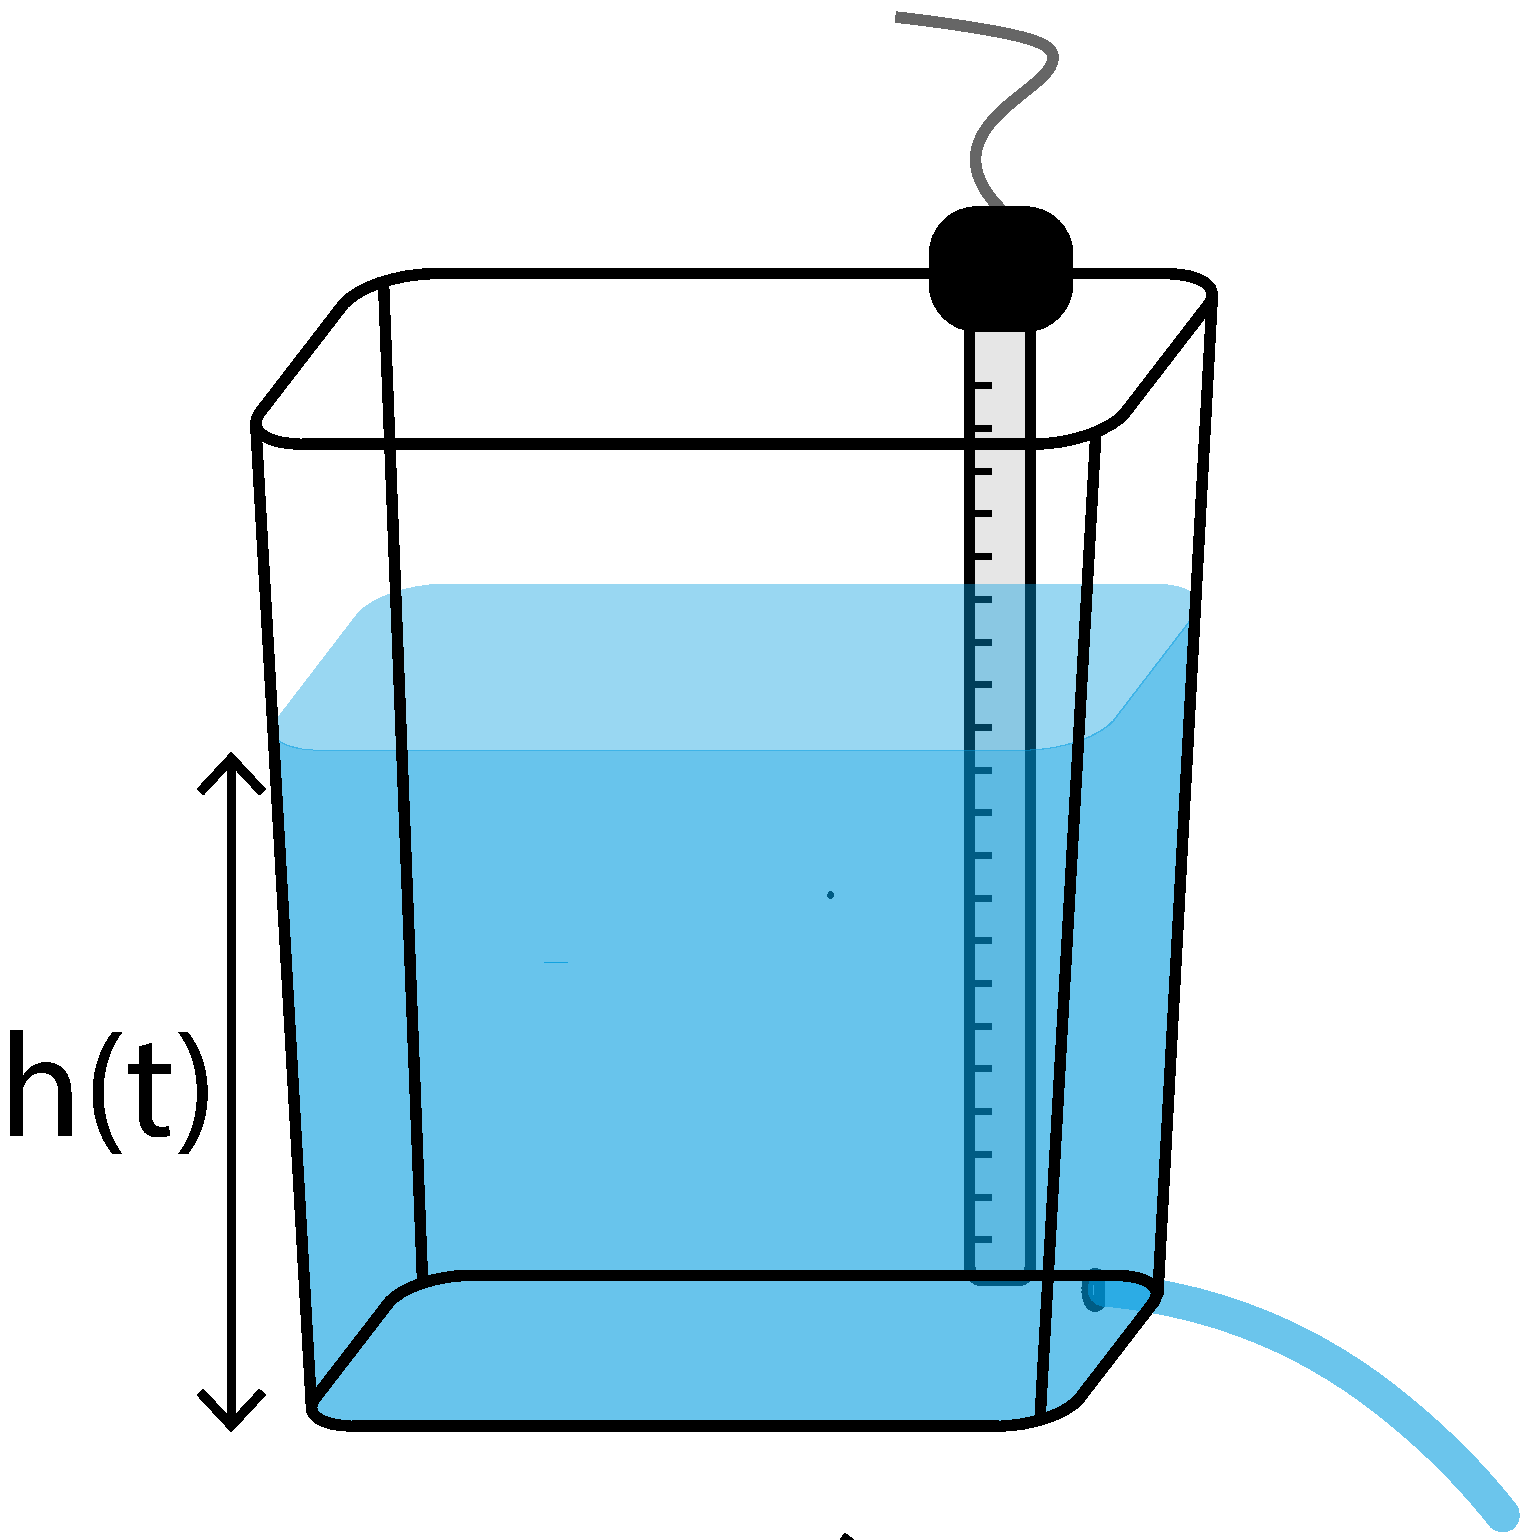
\includegraphics[width=\textwidth]{../tank_geometry/naked_tank.pdf}
	\caption{Experiment setup} \label{fig:naked_tank}
    \end{subfigure}
    
     \begin{subfigure}[b]{0.4\textwidth}
    	\includegraphics[width=\textwidth]{../prior_train.pdf}
	\caption{Prior distribution} \label{fig:prior_train}
    \end{subfigure}
     \begin{subfigure}[b]{0.4\textwidth}
    	\includegraphics[width=\textwidth]{../posterior_train.pdf}
	\caption{Data \& posterior distribution} \label{fig:posterior_train}
    \end{subfigure}
    
     \begin{subfigure}[b]{\textwidth}
     \center
    	\includegraphics[width=0.74\textwidth]{../posterior_train_theta.pdf}
	\includegraphics[width=0.35\textwidth]{../posterior_cov_matrix.pdf}
	\caption{Posterior distribution} \label{fig:posterior_train_theta}
    \end{subfigure}
    \caption{
      \textbf{Model calibration.}
      (a) We fill our empty tank with water, then, at $t=0$, allow it to drain through the orifice in its side.
      (b) Samples of water level trajectories \themodel from the prior probability density $\pi_{\text{pr}}(\thevars)$.
      (c) Time series data \thedata from the tank drainage experiment and samples of water level trajectories \themodel from the posterior distribution $\pi_{\text{post}}(\thevars \mid \thedatanomath)$.
      (d) Visualizing the posterior distribution $\pi_{\text{post}}(\thevars \mid \thedatanomath)$. Top: marginals. Bottom: covariance matrix.      
      }
\end{figure}

\paragraph{The calibrated model.} The forward and measurement models in eqn.~\ref{eq:forward_model} and \ref{eq:H_obs_distn} together with the posterior distribution $\pi_{\text{post}}(\boldsymbol \theta, \boldsymbol \sigma^2 \mid \thedatanomath)$ (with $h_0$ marginalized out and $\boldsymbol \alpha=\mathbf{0}$) constitute the \emph{calibrated model}.
 The calibrated model will be useful for solving the reconstruction problem in phase II, because the presence of an object inside the tank presumably does not affect the parameter vector $\boldsymbol \theta$ nor the measurement noise variance $\sigma^2$ of the level sensor.
We may approximate the posterior distribution as a multi-variate Gaussian distribution
\begin{equation}
	\begin{bmatrix} \boldsymbol \Theta \\ \Sigma \end{bmatrix} \mid \thedatanomath \sim \mathcal{N}(\mathbf{m}, \mathbf{C}) \label{eq:post_theta_sigma}
\end{equation}
with mean $\mathbf{m}$ and covariance matrix $\mathbf{C}$ computed from our MCMC samples $(\boldsymbol \theta_i, \sigma_i)$ from the posterior distribution. 
The means of each parameter in $\mathbf{m}$ and the covariance matrix $\mathbf{C}$ are displayed in Fig.~\ref{fig:posterior_train_theta}. 

\subsubsection{A test experiment}
Before moving onto the reconstruction problem, we test our calibrated model for its ability to predict the dynamics of the liquid level in our tank in a replicate experiment.

We conduct a new, replicate tank-draining experiment (also without an object inside, so $\boldsymbol \alpha=\mathbf{0}$) with measured initial water level $h_{0, \text{obs}}=26.49$\,cm. 
We employ the empirical posterior distribution of $\boldsymbol \Theta$ and $\Sigma^2$ together with $H_0\sim \mathcal{N}(h_{0, \text{obs}}, \sigma^2)$ to sample liquid level trajectories \themodel predicted by the calibrated forward model. 
Fig.~\ref{fig:test} compares the water level time series data collected from the replicate experiment, \thedata, with the trajectories \themodel predicted by the calibrated model. We observe good agreement between the predictions by the calibrated model and the experimental data; the mean absolute residual is 0.28\,cm. (Just for kicks, we show the distribution of predicted tank-emptying times as well.)

\begin{figure}[h!]
    \centering
    	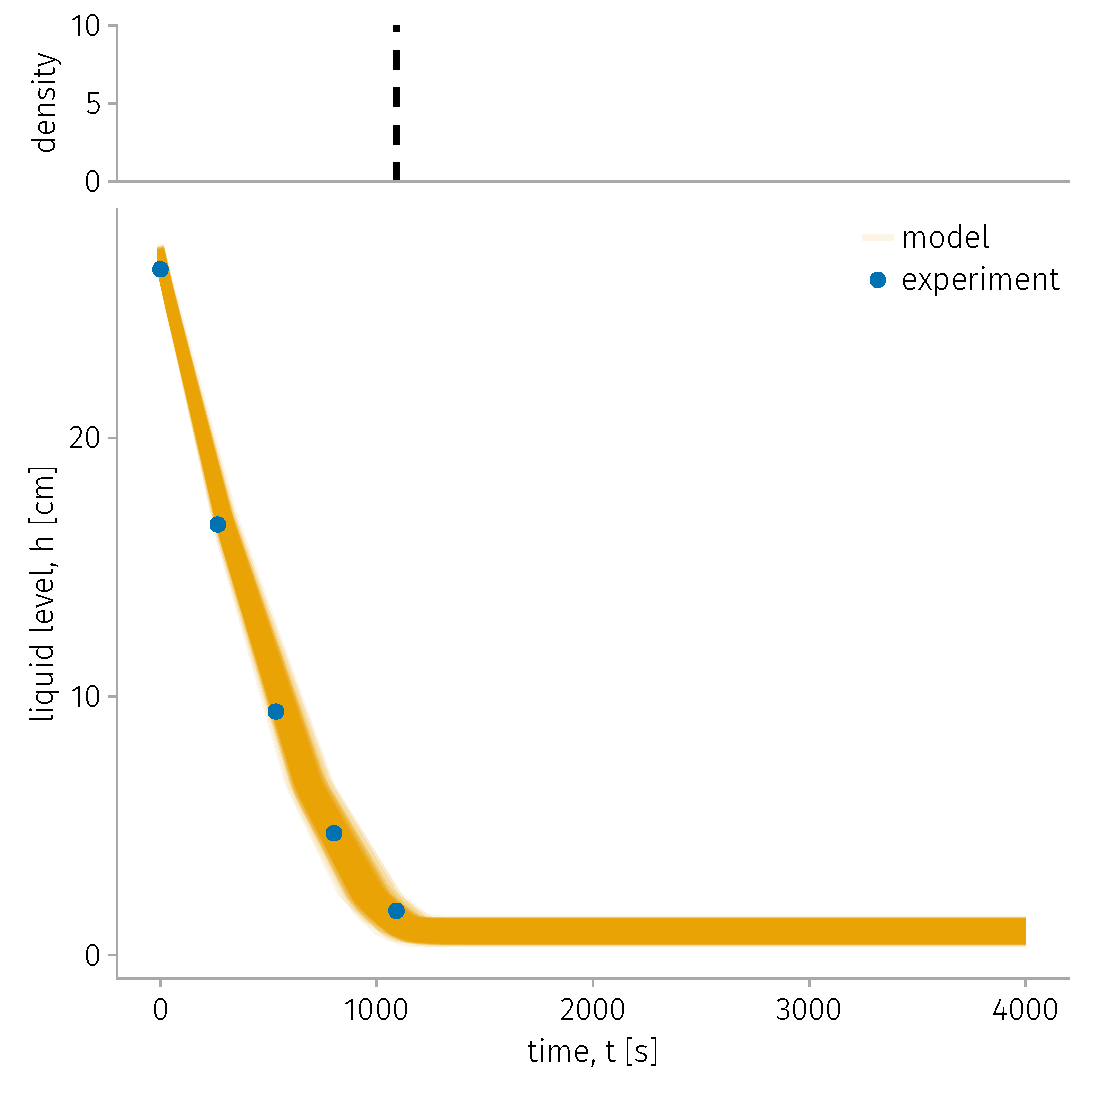
\includegraphics[width=0.5\textwidth]{../test.pdf}
    \caption{
      \textbf{Testing the calibrated forward model.}
      In a replicate tank-draining experiment without an object, we show (top) the predicted distribution of emptying times and (bottom) the water level time series data together with samples of the liquid level trajectory predicted by the calibrated forward model. Note, besides the measured initial water level, the time series data was held out from the model predictions and thus serves as test data.
      } \label{fig:test}
\end{figure}

\subsection{Phase II: Bayesian inference of the shape of an object inside the tank} \label{sec:phaseII}
Finally, we exploit our calibrated model to infer the shape of a heavy, solid object placed in inside of our tank from water level time series data as the tank drains.
Specifically, our objective is to obtain the posterior distribution of $\mathbf{A}$ that characterizes the cross-sectional area of the object as a function of height, $\alpha(h)$ (see eqn.~\ref{eq:alpha}).
This constitutes a reconstruction inverse problem---we aim to reconstruct the input from the observed output.

\subsection{Experimental setup}
We set up a tank draining experiment (see Sec.~\ref{sec:expt}) by:
(i) placing a heavy, solid object inside of the tank, which remains stationary---a large glass bottle;
(ii) fill the tank to an initial water level (measured by the level strip) of $h_{0, \text{obs}}=26.49$\,cm. 
See Fig.~\ref{fig:tank_w_bottle}.


\subsection{Prior distributions}
Our prior distribution for (i) the initial water level $H_0$ is informed by the initial water level measurement; (ii) the parameter vector $\boldsymbol \Theta$ and measurement noise variance $\Sigma^2$ is informed by the model calibration phase; and (iii) the object area $\mathbf{A}$ (a) is diffuse, to entertain a large range of possible object shapes in the tank, and (b) promotes a smooth function $\alpha(h)$. Fig.~\ref{fig:prior_area} displays samples from the prior distribution for the object shape vector $\mathbf{A}$. 

\vspace{-\baselineskip}
\paragraph{The parameter vector and measurement noise variance.}
Abiding by the adage ``yesterday's posterior is today's prior'' \cite{calvetti2010subjective}, we impose a prior distribution on the model parameter vector $\boldsymbol \Theta$ and measurement noise variance $\Sigma^2$ derived from the posterior distribution from our model calibration phase. 
Particularly---we exploit our calibrated forward model by employing as our prior distribution for $\boldsymbol \Theta$ and $\Sigma^2$ the multi-variate Gaussian in eqn.~\ref{eq:post_theta_sigma}.

\vspace{-\baselineskip}
\paragraph{Initial water level.} We impose an informative prior distribution on the initial water level based on the initial reading of the water level sensor:
\begin{equation}
	H_0 \sim \mathcal{N}(h_{0, \text{obs}}, \sigma^2),
\end{equation} where $\sigma^2$ is the variance of the noise from the level sensor in our measurement model.

\vspace{-\baselineskip}
\paragraph{Shape of the object.}
Our prior assumptions about the shape of the object in the tank are:
(i) generally regarding its size, we equally entertain possibilities ranging from the absence of an object to the presence of an object that displaces all water in the tank and
(ii) the cross-sectional area of the object as a function of height, $\alpha(h)$, is a relatively smooth function.

For the diffuse prior over the general size of the object, we impose a uniform distribution on the cross-sectional area of the object at $h=0$, $A_0$ (the random variable representing $\alpha(0)$):
\begin{equation}
	A_0 \sim \mathcal{U}(0, A_b).
\end{equation}
That is, the area of the bottom base of the object could range from zero (no object) to that of the bottom of the tank (largest that can fit in the tank). We are adopting the principe of indifference to allow the water level time series data to ``speak for itself''. 

We sequentially correlate the remainder of the random variables characterizing the object's area, $A_1, ..., A_n$, via a smoothness prior \cite{calvetti2018inverse}: 
\begin{equation}
 A_i - A_{i-1} \sim \mathcal{N}(0, \gamma^2) \text{ for } i \in \{1, ..., n\}.
\end{equation} 
The zero mean Gaussian distribution on the difference of two adjacent object areas means we expect the function $\alpha(h)$ to be flat and change slowly. 
The variance $\gamma^2$ controls the smoothness of $\alpha(h)$; smaller $\gamma^2$ means we expect a smaller difference between adjacent areas and thus a more smooth $\alpha(h)$. 


\subsection{Water level time series data from a tank-drainage experiment}
At time $t:=0$, we allow our tank to drain of water through the small orifice in its side. The liquid level sensor records the water level in the tank over time. The resulting water level time series data \thedata are shown in Fig.~\ref{fig:posterior_object}.

\subsection{Posterior distribution}
Given our (i) prior probability density $\pi_{\text{pr}}(h_0, \boldsymbol \alpha, \boldsymbol \theta, \sigma^2)$---informed for $H_0$, $\boldsymbol \Theta$, and $\Sigma^2$ and diffuse but smooth for $\mathbf{A}$---and (ii) tank drainage data \thedata, from which we construct the likelihood function in eqn.~\ref{eq:like}, the posterior distribution $\pi_{\text{post}}(h_0, \boldsymbol \alpha, \boldsymbol \theta, \sigma^2 \mid \thedatanomath)$ follows from Bayes's theorem in eqn.~\ref{eq:post}. 
We employ the MCMC sampler, NUTS, to obtain samples $\{(h_{0,i}, \boldsymbol \alpha_i, \boldsymbol \theta_i, \sigma^2_i\}$ from the posterior distribution. 

As a posterior predictive check, Fig.~\ref{fig:posterior_object} displays samples of liquid level trajectories \themodel from the posterior distribution. The liquid level trajectories match the time series data reasonably well (mean absolute residual: 0.35\,cm). 

Finally, Fig.~\ref{fig:posterior_area} shows the solution to the reconstruction problem: samples of the object area over different heights, $\mathbf{A}$, from the posterior distribution. Our direct measurements of the area of the object at different heights, using a measuring tape, are plotted as points. Note, this data was held-out from the reconstruction problem; the mean residual between the measured and predicted object area is 7.2\,cm$^2$.
For perspective, posterior samples of the tank area $a(h)$ are shown as well. 
First, the lower variance in $\alpha(h)$ samples from the posterior compared to from the prior (Fig.~\ref{fig:prior_area}) indicates the amount of information the time series data provide about the object's shape. 
Second, the posterior distribution over $\alpha(h)$ agrees reasonably well with the measured area of the object. The data fall within the range of the posterior distribution, but some bias is present in the range $h\in[15, 20]$\,cm. 
Third, note the greater variance in the posterior over the object's area for $h<h_o$ and $h>H$ because it is fundamentally impossible for the water level time series data to provide information about the object's area at those heights; here, the smoothness prior restricts the variance of the predicted area. 
 
\begin{figure}[h!]
    \centering
        \begin{subfigure}[b]{0.3\textwidth}
    	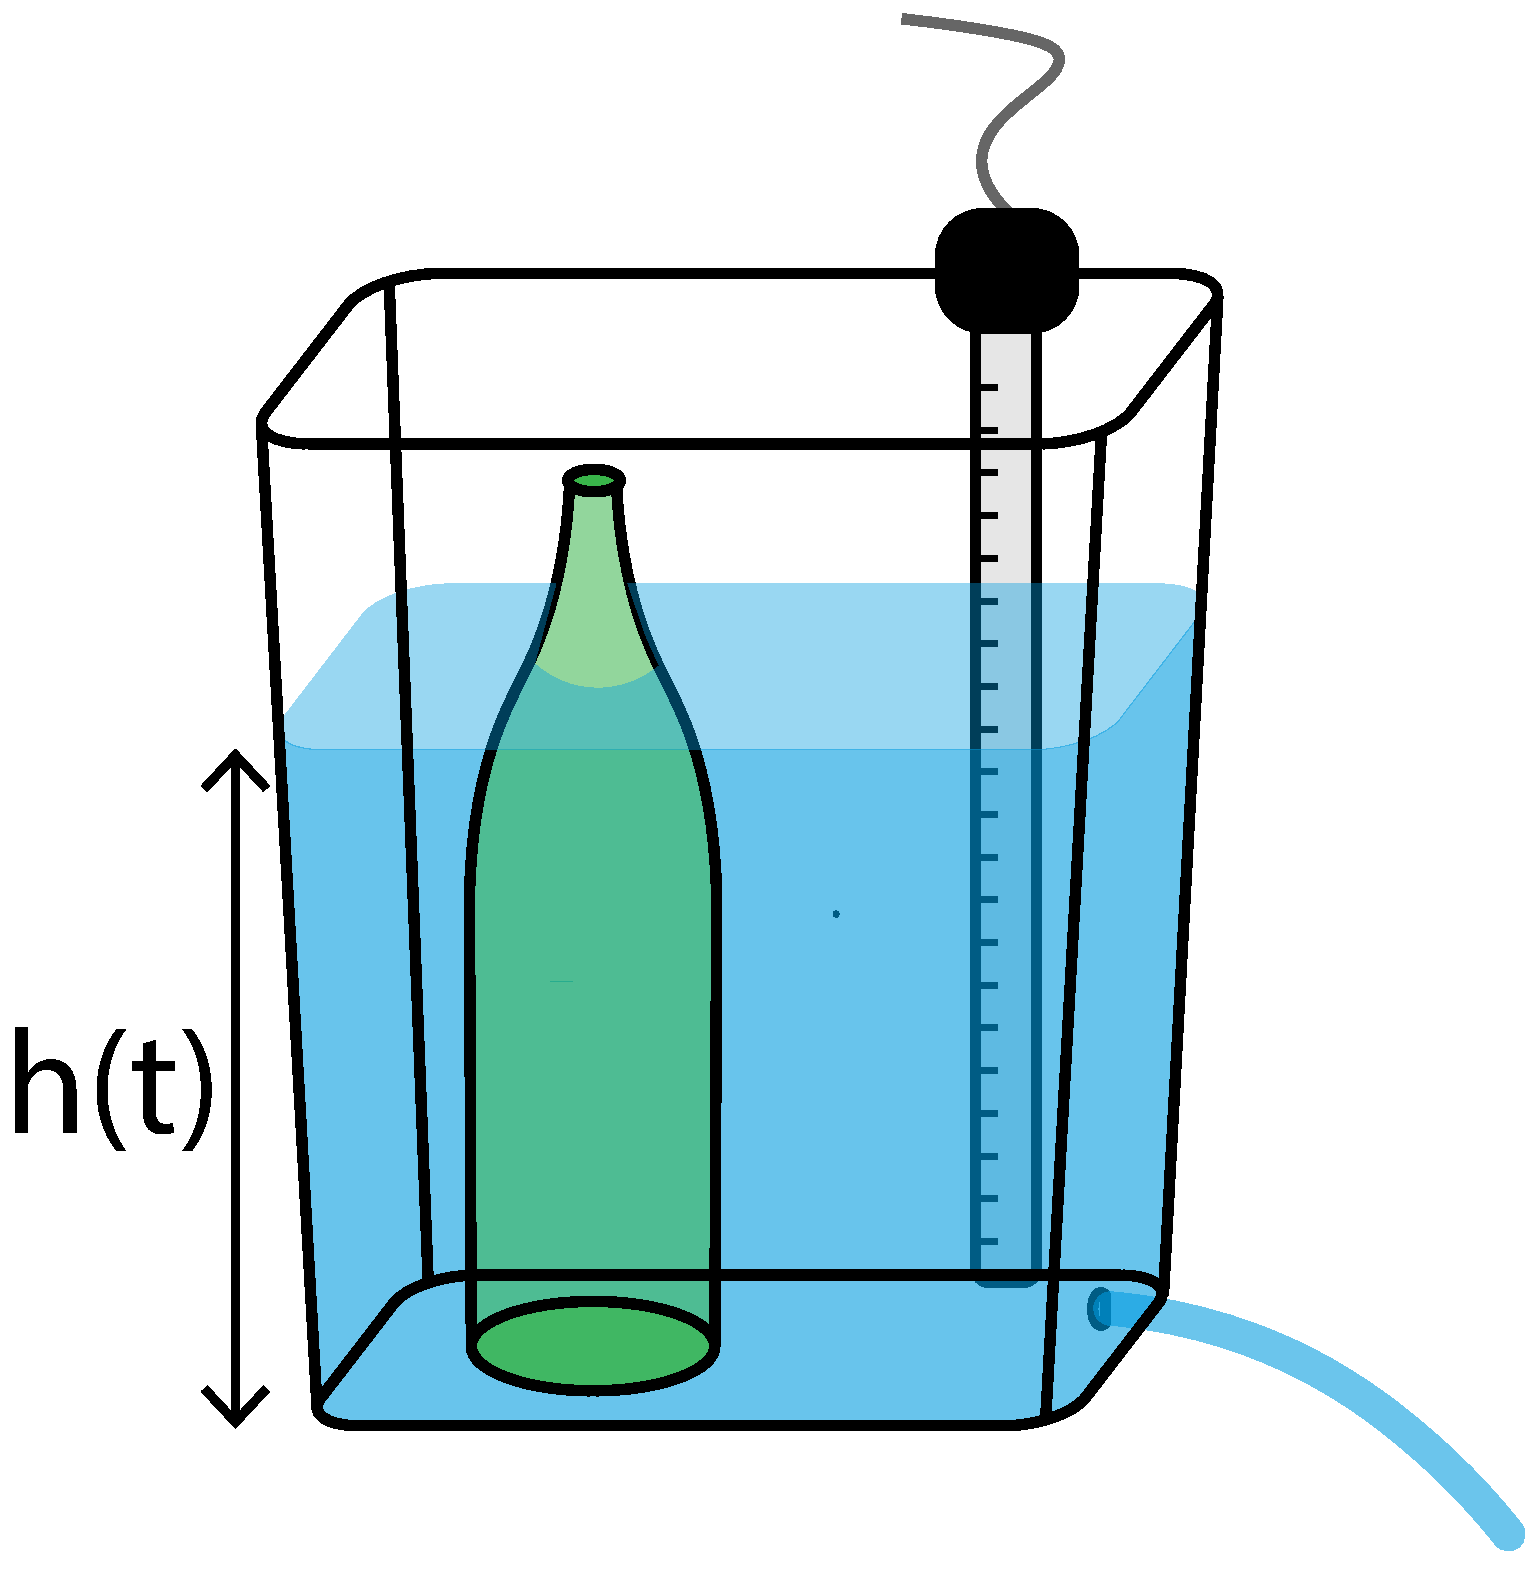
\includegraphics[width=\textwidth]{../tank_geometry/tank_w_bottle.pdf}
	\caption{Experimental setup} \label{fig:tank_w_bottle}
    \end{subfigure}
     \begin{subfigure}[b]{0.49\textwidth}
    	\includegraphics[width=\textwidth]{../prior_area.pdf}
	\caption{Prior dist'n of $\alpha(h)$} \label{fig:prior_area}
    \end{subfigure}
    
     \begin{subfigure}[b]{0.49\textwidth}
    	\includegraphics[width=\textwidth]{../posterior_object.pdf}
	\caption{Data $\{(t_i, h_i)\}$ and posterior dist'n of $h(t)$} \label{fig:posterior_object}
    \end{subfigure}
    \begin{subfigure}[b]{0.49\textwidth}
    	\includegraphics[width=\textwidth]{../posterior_area.pdf}
	\caption{Posterior dist'n of $\alpha(h)$} \label{fig:posterior_area}
    \end{subfigure}

    \caption{
      \textbf{Inferring the shape of the object in the tank.} 
      (a) We fill our tank containing a large, heavy, glass bottle with water, then, at $t=0$, allow it to drain through the orifice in its side.
      (b) Samples of the object cross-sectional area $\mathbf{A}$ from the prior distribution, along with the cross-sectional area of the tank (gray) for perspective. 
      (c) Time series data \thedata from the tank drainage experiment and samples of water level trajectories \themodel from the posterior distribution $\pi_{\text{post}}(\thevars \mid \thedatanomath)$.
      (d) Samples of the object cross-sectional area $\mathbf{A}$ from the posterior distribution, along with the cross-sectional area of the tank (gray) for perspective and the measured (held-out) cross-sectional area of the bottle inside the tank. 
      }
\end{figure}

\section{Conclusions and Discussion}

Forward model could be more complicated: (We do not attempt to explicitly model the flow streamlines inside the tank (as in Refs.~\cite{mathew2014numerical,sakri2017numerical}).)

Calibrate first without object. then can infer shape. well calibration can be with object of whatever shape...

Constrain the space of the shape e.g. if we know it's a cylinder or a trapezoid... then vector-representation of the shape differs.

Rocks inside tank. infer type of rock, coupled with packing. Popcorn polymer.

Surface tension dominates keeping the liquid from exiting. Then Torricelli's law not valid. Liquid stops emptyhing slightly above the hole. 

basis functions for a(h), instead of point by point, but prior harder to interpret.

Mariotte's bottle \cite{kirevs2006mariotte}

\enlargethispage{20pt}

\ack{GF acknowledges ARMI for funding.}

\section{Supporting Information}
\subsection{The liquid level sensor.} 
\label{sec:liq_level_sensor}
We place an immersed, electrical-resistance-based eTape\texttrademark\xspace liquid level strip vertically inside the tank to measure the water level in the tank over time. The liquid level sensor, immersed in the water, communicates with an Arduino microcontroller, allowing us to automatically collect the time series data and write it to a file. The liquid level strip functions by virtue of being compressed by the hydrostatic pressure of the water in which it immersed; its resistive output is inversely proportional to the water level. 
\cite{eTape}
We constructed a calibration curve with a resolution of 1 cm to map the reading from the level sensor [0-1023 integer values] to the liquid level in the tank [cm]. 


%%%%%%%%%% Insert bibliography here %%%%%%%%%%%%%%

\vskip2pc


\bibliographystyle{RS} %%%% .BST file

\bibliography{refs} %%%%% .Bib file

\end{document}
